% !TeX root = ../solution.tex

\hypertarget{he22.30}{%
\chapter{[HE22.30] Jupiter Two}\label{he22.30}}

\begin{marginfigure}
	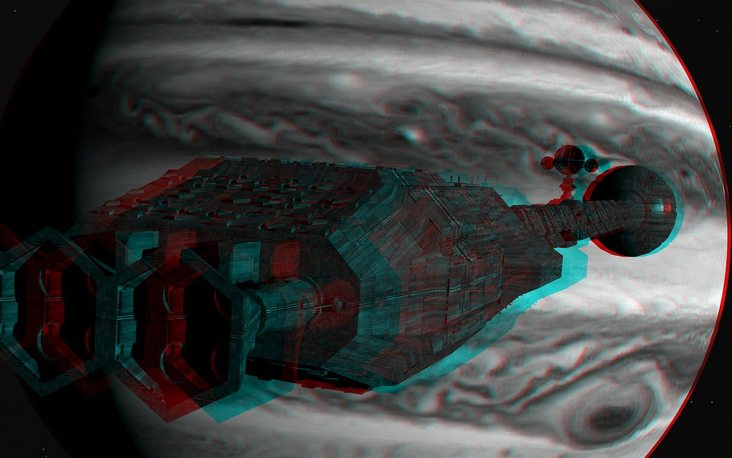
\includegraphics[width=49mm]{level7/challenge30.jpg}
\end{marginfigure}
\section{Intro}
Jupiter is hiding even more.

This time, it is a bit more tricky.

File: \verb+jupiter-two.png+
\subsection{Hint}
Still LSB, but a bit off.

\section{Solution}\label{hv22.30solution}

The picture is of a cyan-red 3D variety and in retrospect it is a hint towards the colours where the flag is hidden.  From the hint it is clear that we have to look again at the LSB of the colour channels, but the hint also tells us that it will not be straight forward.

Several options were tried, but basically all made use of the crib \verb+he2022{+ to identify bit pattern in the colour channels.  To this end a python script was written to extract the LSBs of the channels, convert them into binary strings, and then scan them for occurrences of the patterns.

The crib can then be assumed to be split into two or three colours and thus giving bit patterns that contain every other or every third bit of the crib.  Using only two colours, we find that the red and blue channel match and stippling the two colours together shows the flag \verb+he2022{jupiter_haz_a_great_red_spot!}+
